\section{Symmetric Monoidal Bicategories}
\label{sec:constr-symm-mono}

In this section we will discuss how the iconic functor $\mathcal{H}$ from the previous section extends to a functor of locally cubical bicategories. Furthermore, we will show that it preserves the monoidal structure functorially. We will do this by proving that the functor preserves products, and that every product preserving functor defines a functor between the respective locally cubical bicategories of monoidal cells. 

Note that there are several related notions of these locally cubical bicategories, depending on whether we want the functors to be lax monoidal, oplax monoidal, or strongly monoidal. We will discuss the lax case in this section. In the next section we will generalise this result. We require transformations in $\mathcal{D}bl$ to be horizontally strong.  

%t was shown in~\cite{gg:ldstr-tricat} that tricategories, lax homomorphisms, ico-icons and pseudo-icons form a locally cubical bicategory. As a monoidal bicategory is a tricategory with one object, it follows that monoidal bicategories, lax monoidal functors, lax icons and lax transformations form a locally cubical bicategory as well. 
Double categories, pseudo double functors and tight transformations form a locally cubical bicategory with identity loose 2-cells and identity 3-cells. The functor $\comp$ is defined on tight transformations as the Godement product. The pseudo functor $\compI_A: * \rightarrow \cD bl(A,A)$ maps the cells in the trivial double category $*$ to the identity cells and morphisms in $\cD bl(A,A)$. 

As described in~\cite{gg:ldstr-tricat}, bicategories, pseudo functors, pseudo transformations, icons and cubical modifications also form a locally cubical bicategory. We will recall the definition of icons and cubical modifications.

[insert definition icon]

% By globular tight transformations, we  mean tight transformations $\alpha: F \rightarrow G$ between two functors that agree on objects, such that the family $\{\alpha_f\}$ consists of globular 2-cells. A cubical double modification is defined analogously to a cubical modification~\cite{gg:ldstr-tricat}.

\begin{defn}
Let $F,G,H,K: \D \rightarrow \E$ be pseudo functors; let $\alpha: F \looseRightarrow G$, $\beta: H \looseRightarrow K$ be pseudo transformations; let $\gamma: F \looseRightarrow H$, $\delta: G \looseRightarrow K$ be icons. A cubical modification

\begin{tikzpicture}
\node (tl) at (0,1) {$F$};
\node (tr) at (1,1) {$G$};
\node (bl) at (0,0) {$H$};
\node (br) at (1,0) {$K$};
\draw[doubleloose] (tl) to node[above]{$\alpha$} (tr);
\draw[doubleloose] (bl) to node[below]{$\beta$} (br);
\draw[doubletight] (tl) to node[left]{$\gamma$} (bl);
\draw[doubletight] (tr) to node[right]{$\delta$} (br);
\node at (.5,.5) {$\DDownarrow \Gamma$};
\end{tikzpicture}

is given by a family of 2-cells $\Gamma_A: \alpha_A \RRightarrow \beta_A$ such that for every 1-cell $f:A \rightarrow B$ of $\D$, the following equality holds.

 \begin{equation}
 \begin{aligned}
 \begin{tikzpicture}[scale=1.5]
 \node (tl) at (-1,1) {$FA$};
 \node (tm) at (0,1) {$FB$};
 \node (tr) at (1,1) {$GB$};
 \node (bl) at (-1,0) {$FA$};
 \node (bm) at (0,0) {$GA$};
 \node (br) at (01,0) {$GB$};
 \node (bl1) at (-1,-.7){$HA$};  
 \node (bm1) at (0,-.7) {$KA$};
 \node (br1) at (1,-.7) {$KB$}; 
 \draw[doubleloose] (tm)  to node[above]{$\alpha_B$} (tr);
 \draw[doubleeq] (bm) to (bm1);
 \draw[doubleloose] (bm) to node[above] {$Gf$}(br);
 \draw[doubleeq] (tr) to (br);
 \draw[doubleeq] (tl)  to  (tm);
 \draw[doubleeq] (tl) to (bl);
 \draw[doubleloose] (tl) to node[above]{$Ff$}(tm);
 \draw[doubleloose] (bl) to node[above]{$\alpha_A$}(bm);
 \node at (0,.5) {\footnotesize $\Downarrow \alpha_f$}; 
 \node at (0.5,-.3) {\footnotesize $\Downarrow \delta_f$}; 
  \node at (-0.5,-.3) {\footnotesize $\Downarrow \Gamma_A$};
 \draw[doubleloose] (bl1)  to node[above]{$\beta_A$} (bm1);
 \draw[doubleloose] (bm1) to  node[above]{$Kf$}(br1);
 \draw[doubleeq] (bl)  to (bl1);
 \draw[doubleeq] (br)  to (br1);
 \end{tikzpicture}
 \end{aligned}
 =
\begin{aligned}
 \begin{tikzpicture}[scale=1.5]
 \node (tl) at (-1,1) {$FA$};
 \node (tm) at (0,1) {$FB$};
 \node (tr) at (1,1) {$GB$};
 \node (bl) at (-1,0) {$HA$};
 \node (bm) at (0,0) {$HB$};
 \node (br) at (01,0) {$KB$};
 \node (bl1) at (-1,-.7){$HA$};  
 \node (bm1) at (0,-.7) {$KA$};
 \node (br1) at (1,-.7) {$KB$}; 
 \draw[doubleloose] (tm)  to node[above]{$\alpha_B$} (tr);
 \draw[doubleeq] (tm) to (bm);
 \draw[doubleloose] (bm) to node[above] {$\beta_B$}(br);
 \draw[doubleeq] (tr) to (br);
 \draw[doubleeq] (tl)  to  (tm);
 \draw[doubleeq] (tl) to (bl);
 \draw[doubleloose] (tl) to node[above]{$Ff$}(tm);
 \draw[doubleloose] (bl) to node[above]{$Hf$}(bm);
 \node at (-0.5,.5) {\footnotesize $\Downarrow \gamma_f$}; 
 \node at (0.5,.5) {\footnotesize $\Downarrow \Gamma_B$}; 
 \draw[doubleloose] (bl1)  to node[above]{$\beta_A$} (bm1);
 \draw[doubleloose] (bm1) to  node[above]{$Kf$}(br1);
 \draw[doubleeq] (bl)  to (bl1);
 \draw[doubleeq] (br)  to (br1);
 \node at (0,-0.3) {\footnotesize $\DDownarrow \beta_f$}; 
 \end{tikzpicture}
 \end{aligned}
\end{equation}

\end{defn}

The pseudo functor $\compI_A: * \rightarrow \cB icat(A,A)$ maps the cells in the trivial bicategory $*$ to the identity cells and morphisms of $\cB icat(A,A)$. 
The pseudofunctor $\comp$ is defined on functors and icons as composition in the iconic tricategory $\cB icat$, on pseudo transformations and icons as the Godement product. On cubical modifications it is defined below:

\begin{equation*}
\begin{aligned}
 \begin{tikzpicture}[scale=2]
 \node (tl) at (-1,1) {$FF'A$};
 \node (tm) at (0,1) {$GF'A$};
 \node (tr) at (1,1) {$GG'A$};
 \node (bl) at (-1,0) {$HF'A$};
 \node (bm) at (0,0) {$KF'A$};
 \node (br) at (01,0) {$KG'A$};
 \node (bl1) at (-1,-1){$HH'A$};  
 \node (bm1) at (0,-1) {$KH'A$};
 \node (br1) at (1,-1) {$KK'A$}; 
 \draw[doubleloose] (tm)  to node[above]{$G(\alpha'_A)$} (tr);
 \draw[doubleeq] (tm) to (bm);
 \draw[doubleloose] (bm) to node[above] {$K(\alpha'_A)$}(br);
 \draw[doubleeq] (tr) to (br);
 \draw[doubleeq] (tl)  to  (tm);
 \draw[doubleeq] (tl) to (bl);
  \draw[doubleeq] (bm) to (bm1);
 \draw[doubleloose] (tl) to node[above]{$\alpha_{F'A}$}(tm);
 \draw[doubleloose] (bl) to node[above]{$\beta_{F'A}$}(bm);
 \node at (-0.5,.5) {\footnotesize $\Downarrow \Gamma_{F'A}$}; 
 \node at (0.5,.5) {\footnotesize $\Downarrow \delta_{\alpha'_A}$}; 
 \draw[doubleloose] (bl1)  to node[above]{$\beta_{H'A}$} (bm1);
 \draw[doubleloose] (bm1) to  node[above]{$K(\beta'A)$}(br1);
 \draw[doubleeq] (bl)  to (bl1);
 \draw[doubleeq] (br)  to (br1);
 \node at (-.5,-0.5) {\footnotesize $=$}; 
\node at (.5,-0.5) {\footnotesize $\DDownarrow K\Gamma'_A$}; 
\end{tikzpicture}
\end{aligned}
\end{equation*}
%%%%%%%%%

If $\gamma_{\transid} = \delta_{\transid} = \tightid$, functoriality follows from naturality of the icons. Note that there are several canonical ways to define this composition on cubical modifications, by choosing different versions of the Godement product.  

For $\cB icat$ and $\cD bl$, all identity cells are lax monoidal. In fact, all identity cells are strong monoidal braided, sylleptic and symmetric. This means that the requirements from the previous section is satisfied; hence, the locally cubical bicategories $\cMon \cDbl$ and $\cMon \cBicat$ of monoidal cells and morphisms of $\cDbl$ and $\cBicat$, respectively, are well-defined.

Monoidal double categories, monoidal pseudo functors and monoidal tight transformations form a locally cubical bicategory with identity loose 2-cells and 3-cells.

We upgrade the functor from theorem 4.11 to a functor of locally cubical bicategories.


\begin{defn}\label{def:lcbcfunc}
Let ${\bf S,T}$ be locally cubical bicategories. A functor $\cT: {\bf T} \rightarrow {\bf S}$ consists of the following data:
\begin{enumerate}
\item An assignment on objects that sends each object $A$ of ${\bf T}$ to an object $\cT A$ of ${\bf S}$.
\item For each two objects $A,B$, a pseudo double functor (1-cell in \cDbl) ${\bf T}(A,B) \rightarrow {\bf S}(\cT(A),\cT(B))$
\item For every triple of objects $A,B,C$ of ${\bf T}$, a tight transformation (2-cell in $\cD bl$) 
\begin{align} 
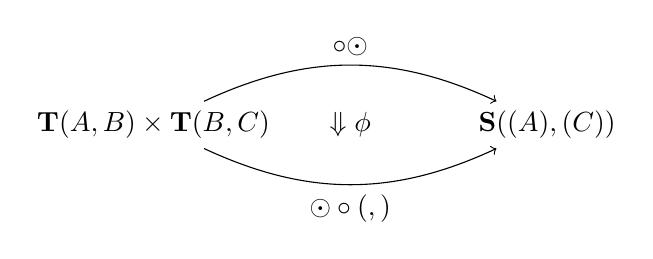
\begin{tikzpicture}
\node(1) at (0,0) {${\bf T}(A,B) \times {\bf T}(B,C)$};
\node(2) at (5,0) {${\bf S}(\cT(A),\cT(C))$};
\draw[->] (1) to[in=155, out=25] node[above]{$\cT \circ \odot$} (2); 
\draw[->] (1) to[in=-155, out=-25] node[below]{$\odot \circ (\cT,\cT)$} (2); 
\node at (2.5,0) {$\Downarrow \phi \iso$};
\end{tikzpicture}
\end{align}
where $\odot$ denotes horizontal composition.
\item For every object $A$ of {\bf T} a tight transformation
\begin{align}
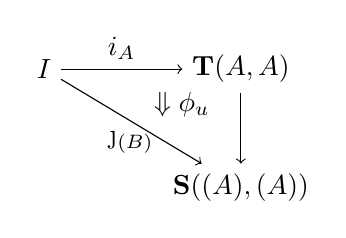
\begin{tikzpicture}[xscale=.5, yscale=.3]
\node(1) at (0,0) {$I$};
\node(2) at (5,0) {${\bf T}(A,A)$};
\node(3) at (5,-5) {${\bf S}(\cT(A),\cT(A))$};
\draw[->] (1) to node[above]{$i_{A}$} (2); 
\draw[->] (1) to node[below]{$\j_{\cT(B)}$} (3);
\draw[->] (2) to node[right]{$\cT$} (3); 
\node at (3.5,-1.5) {$\Downarrow \phi_u \iso$};
\end{tikzpicture}
\end{align}
where $i$ and $j$ are the unitors of ${\bf S}$ and ${\bf T}$.
\item The usual coherence diagrams, Definition 10 of~\cite{nick:tricatsbook} commute.
\end{enumerate}
\end{defn}



\begin{thm}
The iconic functor $\cH: \cD bl_{\bf f} \rightarrow \cB icat$ extends to a functor of locally cubical bicategories.
\end{thm}

\begin{thm}
The functor   $\cH: \cD bl_{\bf f} \rightarrow \cB icat$ of locally cubical bicategories preserves products.
\end{thm}

 \begin{lem}
  Let ${\bf S,T}$ be locally cubical bicategories with products. Any functor $\mathcal{T}: T \rightarrow S$ that preserves products, preserves  monoidal objects, 1-cells, 2-cells, icons and 3-cells as well as any braided, sylleptic or symmetric structure of these objects, 1-cells,2-cells, icons and 3-cells.
 \end{lem}
 
 \begin{proof}
Let $A$ be a monoidal object. As the functor $\mathcal{T}$ preserves products, we have a product $\cT(A) \times_{\cT} \cT(A) = \cT(A \times A)$. As a consequence $\ten\maps
  A\times A\to A$ induces a 1-cell $\ten_{\mathcal{T}} \maps
 \mathcal{T}A\times_{\cT} \mathcal{T} A\to\mathcal{T}A$ with a unit 1-cell $I_{\mathcal{T}}$, where $\cT(f) \ten_{\cT} \cT(g) := \cT(f \ten g)$ and $I_{\cT}:= \mathcal{T}(I)$. 
 
 Note that conditions $(iii)$ and $(iv)$ of definition \ref{def:lcbcfunc} imply that for all 1-cells $f,g$ we have an isomorphism $\cT(f \odot g) \iso \cT(f) \odot \cT(g)$ and for the identity 1-cell we have an isomorphism $\id_A$, $\cT(\id_A) \iso \id_{\cT(A)}$. Hence, the associativity 2-cell of $A$ gives rise to a 2-cell
  \[\vcenter{\xymatrix@C=6pc{\cT(A)\times\cT(A)\times\cT(A) \rtwocell^{\ten_{\cT}
        (\Id\times\ten_{\cT})}_{\ten_{\cT}(\ten_{\cT}\times\Id)}{\hspace{.2cm}\fa_{\cT}\eqv} &\cT(A) }}\]
  which simply equals $\cT(\alpha) $together with the invertible 2-cells [check this, initially it was an equality because of icons. what is the icon-equivalent for double categories?].
  
  Likewise, the unit constraints $l, r$ as well as the constraints for (braided) monoidal 1-cells $\sigma$ induce 1-cells $l_{\cT}, r_{\cT}$, and $\sigma_{\cT}$, respectively.
  
 Furthermore, the invertible 3-cell filling the Mac Lane pentagon lifts to the invertible 3-cell of the Mac Lane Pentagon for $\cT(A)$. Which is simply its image under $\cT$, composed with the isomorphic $3$-cells given by (iii) of definition \ref{def:lcbcfunc}, ensuring that it has the right type.
%   \[\xy
%  (-10,0)*{\ten_{\cT}(\ten_{\cT},\Id)(\ten_{\cT}, \Id, %\Id)}="A";
%  (20,10)*{\ten_{\cT}(\ten_{\cT},\Id)(\Id, \ten_{\cT},\Id)}="B";
%  (50,0)*{\ten_{\cT}(\Id,\ten_{\cT})(\Id, \ten_{\cT},\Id)}="C";
%  (0,-15)*{\ten_{\cT}(\Id, \ten_{\cT})(\ten, \Id, \Id)}="D";
%  (40,-15)*{\ten_{\cT}(\Id, \ten_{\cT})(\Id, \Id, \ten, _{\cT})}="E";
%  (20,-5)*{\scriptstyle\Downarrow \pi \iso};
%  \ar "B";"A";^{\fa_{\cT} \ten_{\cT} \id}
%  \ar "C";"B";^{\fa_{\cT}}
%  \ar "D";"A";_{\fa_{\cT}}
%  \ar "E";"D";_{\fa_{\cT}}
%  \ar "E";"C";^{\id\ten_{\cT} \fa_{\cT}}
%  \endxy
%  \]
  
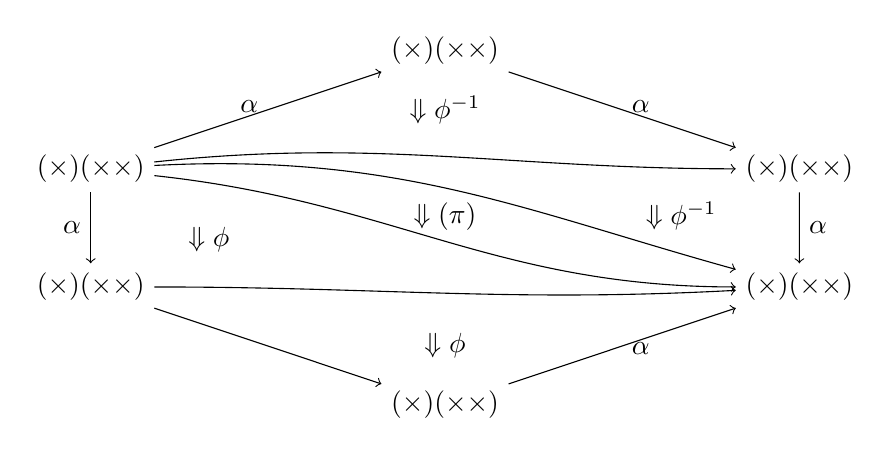
\begin{tikzpicture}[yscale=1.5, xscale=3]
\node(tl) at (0,1) {$\ten (\ten \times \Id)(\ten \times \Id \times \Id)$};
\node(t) at (1.5,2) {$\ten (\ten \times \Id)(\Id \times \ten \times \Id)$};
\node(tr) at (3,1) {$\ten (\Id \times \ten )(\Id \times \ten \times \Id)$};
\node(br) at (3,0) {$\ten (\Id \times \ten )(\Id \times \Id \times \ten )$};
\node(b) at (1.5,-1) {$\ten (\ten \times \Id)(\Id \times \Id \times \ten )$};
\node(bl) at (0,0) {$\ten (\Id \times \ten )(\ten \times \Id \times \Id)$};
\draw[->] (tl) to node[left, yshift=1pt] {$\alpha \ten \id$} (t);
\draw[->] (t) to node[right, yshift=1pt] {$\alpha$} (tr);
\draw[->] (tr) to node[right] {$\id \ten \alpha$} (br);
\draw[->] (tl) to node[left] {$\alpha$} (bl);
\draw[->] (bl) to node[left,yshift=-1pt] {$\id$} (b);
\draw[->] (b) to node[right,yshift=-1pt] {$\alpha$} (br);
\draw[->] (tl) to [in=155, out=5] (br);
\draw[->] (tl) to [in=180, out=-10] (br);
\draw[->] (tl) to [in=180, out=10](tr);
\draw[->] (bl) to [in=185, out=0](br);
\node at (1.5,.6) {$\Downarrow \cT(\pi) \iso$};
\node at (2.5,.6) {$\Downarrow \phi^{-1} \iso$};
\node at (1.5,1.5) {$\Downarrow \phi^{-1} \iso$};
\node at (.5,.4) {$\Downarrow \phi \iso$};
\node at (1.5,-.5) {$\Downarrow \phi \iso $};
\end{tikzpicture}  

 Note that there may be several way to past these 3-cells, but by coherence of pseudofunctors, the result is the same. Likewise, the isomorphic 3-cells $\mu, \lambda,\rho$ and the isomorphic 3-cells $R,S$, and $v$ witnessing the braiding and syllepsis, lift to the appropriate 3-cell for $\cT(A)$. This is also the case for the isomorphic 3-cells $R,S$ that characterise the braiding. 
   Finally, we need to show that the three equations between pasting composites of $\pi_{\cT}, \mu_{\cT}, \lambda_{\cT}, \rho_{\cT}$ hold ???

The argument for 1-cells and 2-cells is similar. 
Let $f,g:A \rightarrow B$ be monoidal 1-cells and let $\alpha: f \Rightarrow g$ be a monoidal 2-cell.
The 2-cells $\chi: \otimes_B \odot (f,f) \Rightarrow f \odot \otimes_A$ and $\iota: I_B \Rightarrow f \odot I_A$ are mapped to $\cT(\chi): \otimes_{\cT(B)} \odot (\cT(f),\cT(f)) \Rightarrow \cT(f) \odot \otimes_{\cT(A)}$ and $\iota: I_{\cT(B)} \Rightarrow \cT(f) \odot I_{\cT(A)}$. Similarly, any 2-cell witnessing a braiding $u: \sigma_B \odot \chi  \Rightarrow \chi \odot f\sigma_A$  is mapped to $\cT(u): \sigma_{\cT(B)} \odot \cT(\chi)  \Rightarrow \cT(\chi) \odot \cT(f)\sigma_{\cT(A)}$.
Analogously to $\alpha$, the invertible 3-cells $\omega, \gamma$, and $\delta$, and $\Pi$ and $M$ are lifted to their images under $\cT$, augmented with instances of $\phi$ to ensure that the 3-cells have the right type.
 It is left to show that the equations pasting composites of these 3-cells together commute.
 \end{proof}
 
TODO: Enhance that to a functor.

\begin{thm}
Any product preserving functor of locally cubical bicategories$F: \cC  \rightarrow \cD$ lift to a functor between the locally cubical bicategories of monoidal objects and lax monoidal cells $ \cM on \cC  \rightarrow \cM on\cD$
\end{thm}


